% *********************************************************************
% © 2010–2026 Jeremy Sylvestre
%
% Permission is granted to copy, distribute and/or modify this document
% under the terms of the GNU Free Documentation License, Version 1.3 or
% any later version published by the Free Software Foundation; with no
% Invariant Sections, no Front-Cover Texts, and no Back-Cover Texts. A
% copy of the license is included in the appendix entitled “GNU Free
% Documentation License” that appears in the output document of this
% PreTeXt source code. All trademarks™ are the registered® marks of
% their respective owners.
%
% *********************************************************************

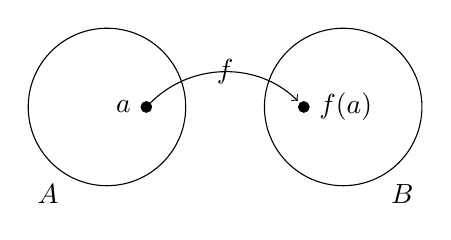
\begin{tikzpicture}[
	vertex/.style={ circle, draw, very thin, fill, inner sep=0pt, minimum size=4pt },
	vertexg/.style={ black!40!white, circle, draw, very thin, fill, inner sep=0pt, minimum size=4pt },
	vertexo/.style={ circle, draw, very thin, inner sep=0pt, minimum size=4pt }
]
	\draw (1.5,0) circle (1cm);
	\draw (-1.5,0) circle (1cm);
	\node at (2.25,-1.1) {$B$};
	\node at (-2.25,-1.1) {$A$};
	\node at (-1,0) (a) [vertex,label=left:$a$] {};
	\node at (1,0) (b) [vertex,label=right:$f(a)$] {};
	\draw[->,shorten >=1pt] (a) to [out=45,in=135] node {$f$} (b);
\end{tikzpicture}
